\documentclass[paper=letter, fontsize=11pt]{scrartcl} 

\usepackage{graphicx}
\usepackage{verbatim}
\usepackage{pictex}  
\usepackage{multimedia}
\usepackage{amsbsy}
\usepackage{amssymb}

\usepackage{listings}
\usepackage{xcolor,colortbl}
\usepackage[spanish]{babel} 
%\usepackage{amsmath} 
\usepackage{amsfonts, amsthm}
\usepackage{fancyvrb}
\usepackage{sectsty} % Allows customizing section commands
\allsectionsfont{\centering \normalfont\scshape} % Make all sections centered, the default font and small caps

\usepackage{fancyhdr} % Custom headers and footers
\pagestyle{fancyplain} % Makes all pages in the document conform to the custom headers and footers
\fancyhead{} % No page header - if you want one, create it in the same way as the footers below
\fancyfoot[L]{} % Empty left footer
\fancyfoot[C]{} % Empty center footer
\fancyfoot[R]{\thepage} % Page numbering for right footer
\renewcommand{\headrulewidth}{0pt} % Remove header underlines
\renewcommand{\footrulewidth}{0pt} % Remove footer underlines
\setlength{\headheight}{13.6pt} % Customize the height of the header

\numberwithin{equation}{section} % Number equations within sections (i.e. 1.1, 1.2, 2.1, 2.2 instead of 1, 2, 3, 4)
\numberwithin{figure}{section} % Number figures within sections (i.e. 1.1, 1.2, 2.1, 2.2 instead of 1, 2, 3, 4)
\numberwithin{table}{section} % Number tables within sections (i.e. 1.1, 1.2, 2.1, 2.2 instead of 1, 2, 3, 4)

\setlength\parindent{0pt} % Removes all indentation from paragraphs - comment this line for an assignment with lots of text

\newcommand{\horrule}[1]{\rule{\linewidth}{#1}} % Create horizontal rule command with 1 argument of height

\title{	
\normalfont \normalsize 
\textsc{Centro de Investigaci\'on en Matem\'aticas (CIMAT). Unidad Monterrey} 
\\ [25pt] 
\horrule{0.5pt} \\[0.4cm] % Thin top horizontal rule
\huge Tarea 1 \\ 
\horrule{2pt} \\[0.5cm] % Thick bottom horizontal rule
}

\author{Enrique Santibáñez Cortés} % Your name

\date{\normalsize\today} % Today's date or a custom date

\begin{document}
\lstdefinestyle{customc}{
  belowcaptionskip=1\baselineskip,
  basicstyle=\footnotesize, 
  frame=lrtb,
  breaklines=true,
  %frame=L,
  %xleftmargin=\parindent,
  language=C,
  showstringspaces=false,
  basicstyle=\footnotesize\ttfamily,
  keywordstyle=\bfseries\color{green!40!black},
  commentstyle=\itshape\color{red!40!black},
  identifierstyle=\color{blue},
  stringstyle=\color{purple},
}

\lstset{breakatwhitespace=true,
  basicstyle=\footnotesize, 
  commentstyle=\color{green},
  keywordstyle=\color{blue},
  stringstyle=\color{purple},
  language=C++,
  columns=fullflexible,
  keepspaces=true,
  breaklines=true,
  tabsize=3, 
  showstringspaces=false,
  extendedchars=true}

\lstset{ %
  language=R,    
  basicstyle=\footnotesize, 
  numbers=left,             
  numberstyle=\tiny\color{gray}, 
  stepnumber=1,              
  numbersep=5pt,             
  backgroundcolor=\color{white},
  showspaces=false,             
  showstringspaces=false,       
  showtabs=false,               
  frame=single,                 
  rulecolor=\color{black},      
  tabsize=2,                  
  captionpos=b,               
  breaklines=true,            
  breakatwhitespace=false,    
  title=\lstname,             
  keywordstyle=\color{blue},  
  commentstyle=\color{dkgreen},
  stringstyle=\color{mauve},   
  escapeinside={\%*}{*)},      
  morekeywords={*,...}         
} 


\maketitle % Print the title

\section{Problema 1}

Concluye el ejercicio de análisis en los datos \textit{olive} según los objetivos que discutimos en clase, es decir, tratar de identificar las regiones de los aceites y también las áreas dentro de  cada región.

\subsection{Solución}

\section{Problema 2}

Considera los datos que se encuentran en el archivo \textit{suicide\_data.csv}, que compila información relacionada con suicidios en 101 países en diferentes años e incluye también algunos indicadores de desarrollo, como el Producto Interno Bruto (GPD) y percapita, Índice de Desarrollo Humano (HDI), entre otra información.

\subsection{a) ¿Qué preguntas de interés puedes formular para analizar éste fenómeno en base a estos datos?}

Considero que las primeras preguntas a contestar serían: \textbf{¿Actualmente los suicidios por año son mayores que hace 20 años? ¿Cómo es la tendencia de los suicidios (o tasa de suicidios) a  nivel mundial?} Esta pregunta es muy general, pero creo que nos daría un mucha información acerca de la importancia que tienen los suicidios actualmente.\\

Ahora, considerando las variables económicas podemos contestar las siguientes preguntas: \textbf{¿Existe una relación entre el desarrollo económico de un país y el número de suicidios(o la tasa de suicidios)?} Claramente se esperaría que si existía una relación, debido a que si consideramos que el desarrollo económico de un país esta asociado en sus recursos que se les asignan a cada sector del país (educación, salud, infraestructura, etc), los países bajo desarrollo económico en donde los recursos para el sector salud es menor esto implicaría que la identificación y el tratamiento de los suicidios sería más escasos que los países con mayor desarrollo económico.\\ 

Y por último, me gustaría contestar lo siguiente: \textbf{¿Existen algún rango de edad en la cuál están las personas a suicidarse? ¿Qué genero esta más propenso a suicidarse? ¿esto es diferente en cada país?} Considero que las personas jóvenes-adultas estarían más propensos a suicidarse, esta hipótesis se basa en que a esa edad no se esta consiente de muchas cosas y es cuando las personas se desarrollan personal y profesionalmente lo que provoca que estén más expuesto a estrés, problemas, etc. Por otro lado, creo que la puede existe una gran diferencia entre los suicidios por genero en cada país, ya que podemos pensar que los países en los que los derechos de las mujeres no sean los adecuados o igualitarios que los hombres esto provoque una diferencia en la tasa de suicidios.\\

Dependiendo de las resultados podemos ampliar las preguntas considerando las variables económicas y las variables de edad y género, pero para no hacer el análisis tan complejo empezaremos con estas preguntas. $\blacksquare$

\subsection{b) Realiza un análisis exploratorio y descriptivo de los datos con las herramientas que consideres apropiadas. ¿Qué estructuras o correlaciones encuentras?}

El índice de desarrollo humano no esta reportado en 22 años específicos (Ver Figura \ref{hdi_null}), lo que se espera que esta variable no sea de gran importancia para este análisis. 

\begin{figure}[h]
    \centering
    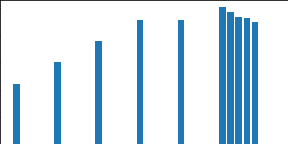
\includegraphics{../figs/dhi_null.png}
    \caption{Total de registros nulos HDI por año}
    \label{hdi_null}
\end{figure}

Ahora, el lapso de tiempo estudiado es de 1985 a 2016 lo equivale un total de 31 años. 24 países tienen menos de 20 años con registros, no se filtraron es debido a que la gran mayoría de los países pertenecen a países con un bajo desarrollo por lo que desequilibraría el conjunto de datos. 



\subsection{c) Trata de responder las preguntas que formulaste en el primer inciso. ¿Puedes obtener conclusiones interesantes?}

Al analizar la tasa de suicidios por 

\subsection{d) Considera solamente los datos de México y Estados Unidos. Realiza los incisos
2$b$ y 2$c$ por separado y compara los resultados. ¿Qué puedes concluir?}

\subsection{e) ¿Qué otra información te gustaría tener disponible para analizar éste fenómeno y cómo la utilizaría?}
\end{document}
